% !TeX spellcheck = en_GB
\documentclass[12pt]{beamer}

\usetheme[sectionpage=none, subsectionpage=progressbar, progressbar=foot, numbering=fraction]{metropolis}

\makeatletter
\setlength{\metropolis@frametitle@padding}{1.6ex}% <- default 2.2 ex

\setbeamertemplate{footline}{%
  \begin{beamercolorbox}[wd=\textwidth, sep=1.5ex]{footline}% <- default 3ex
    \usebeamerfont{page number in head/foot}%
    \usebeamertemplate*{frame footer}
    \hfill%
    \usebeamertemplate*{frame numbering}
  \end{beamercolorbox}%
}
\makeatother

\AtBeginSubsection
{
  \begin{frame}{Where are we?}
    \tableofcontents[sectionstyle=show/shaded, subsectionstyle=show/shaded/hide]
  \end{frame}
}

\makeatletter
\setbeamertemplate{headline}{
  \begin{beamercolorbox}{upper separation line head}
  \end{beamercolorbox}
  \begin{beamercolorbox}{section in head/foot}
    \vskip2pt\insertsectionnavigationhorizontal{\paperwidth}{}{}\vskip2pt
  \end{beamercolorbox}
  \begin{beamercolorbox}{lower separation line head}
  \end{beamercolorbox}
}
\makeatother
\setbeamercolor{section in head/foot}{fg=normal text.bg, bg=structure.fg}

\setbeamertemplate{itemize items}[square]

\usepackage{menukeys}
\usepackage{minted}
\setminted[bash]{fontsize=\small, tabsize=2, breaklines}

\title{
\includegraphics[width=0.5\linewidth]{hackerschool} \\ Hacker Tools: Part 1}
\author{Julius Putra Tanu Setiaji}
\date{23 March 2019}

\begin{document}

\frame[plain]{\titlepage}

\section{Introduction}
\subsection{}

\begin{frame}{NUS Hackers}

  \begin{center}
    
\includegraphics[width=0.5\linewidth]{NUSHackers}

    \url{http://nushackers.org}
  \end{center}

  \begin{center}
    \textbf{hacker}school

    Friday \textbf{Hacks}

    \textbf{Hack} \& Roll

    NUS \textbf{Hacker}space
  \end{center}

\end{frame}

\begin{frame}{About Me}
  Hi! I'm Julius. My GitHub is \url{https://github.com/indocomsoft}

  A Year 2 Computer Science Undergraduate who loves hacking and building systems.

  I also enjoy Space Exploration, Music Theory and History. {\tiny (my favourite games are KSP and EU4 hit me up if you play those too)}
\end{frame}

\begin{frame}{About This Workshop}
  \begin{itemize}
    \item No prior knowledge assumed
    \item Learning how to make the most of tools that productive programmers use.
    \item How to hack on Unix-like environment.
  \end{itemize}
\end{frame}

\begin{frame}
  \frametitle{Table of Contents}
  \tableofcontents[sectionstyle=show/show,subsectionstyle=hide/hide/hide]
\end{frame}

\begin{frame}{Required Software}
  Unix-like environment, either one of these:
  \begin{itemize}
    \item Linux\footnote{For beginners, Ubuntu is recommended. Either dual-boot or install as virtual machine using VirtualBox}
    \item macOS\footnote{Open Terminal, and run \mintinline{bash}{xcode-select --install} first}
    \item BSD
    \item Other Unix-like OS'es (Minix, Solaris, AIX, HP-UX, etc.)
  \end{itemize}
\end{frame}

\begin{frame}{Unix? Can I eat that?}
  \begin{itemize}
    \item A family of multitasking, multiuser OS'es.
    \item First developed in the 1970's.
    \item Popularised the use of interactive command line.
  \end{itemize}
  \begin{center}
    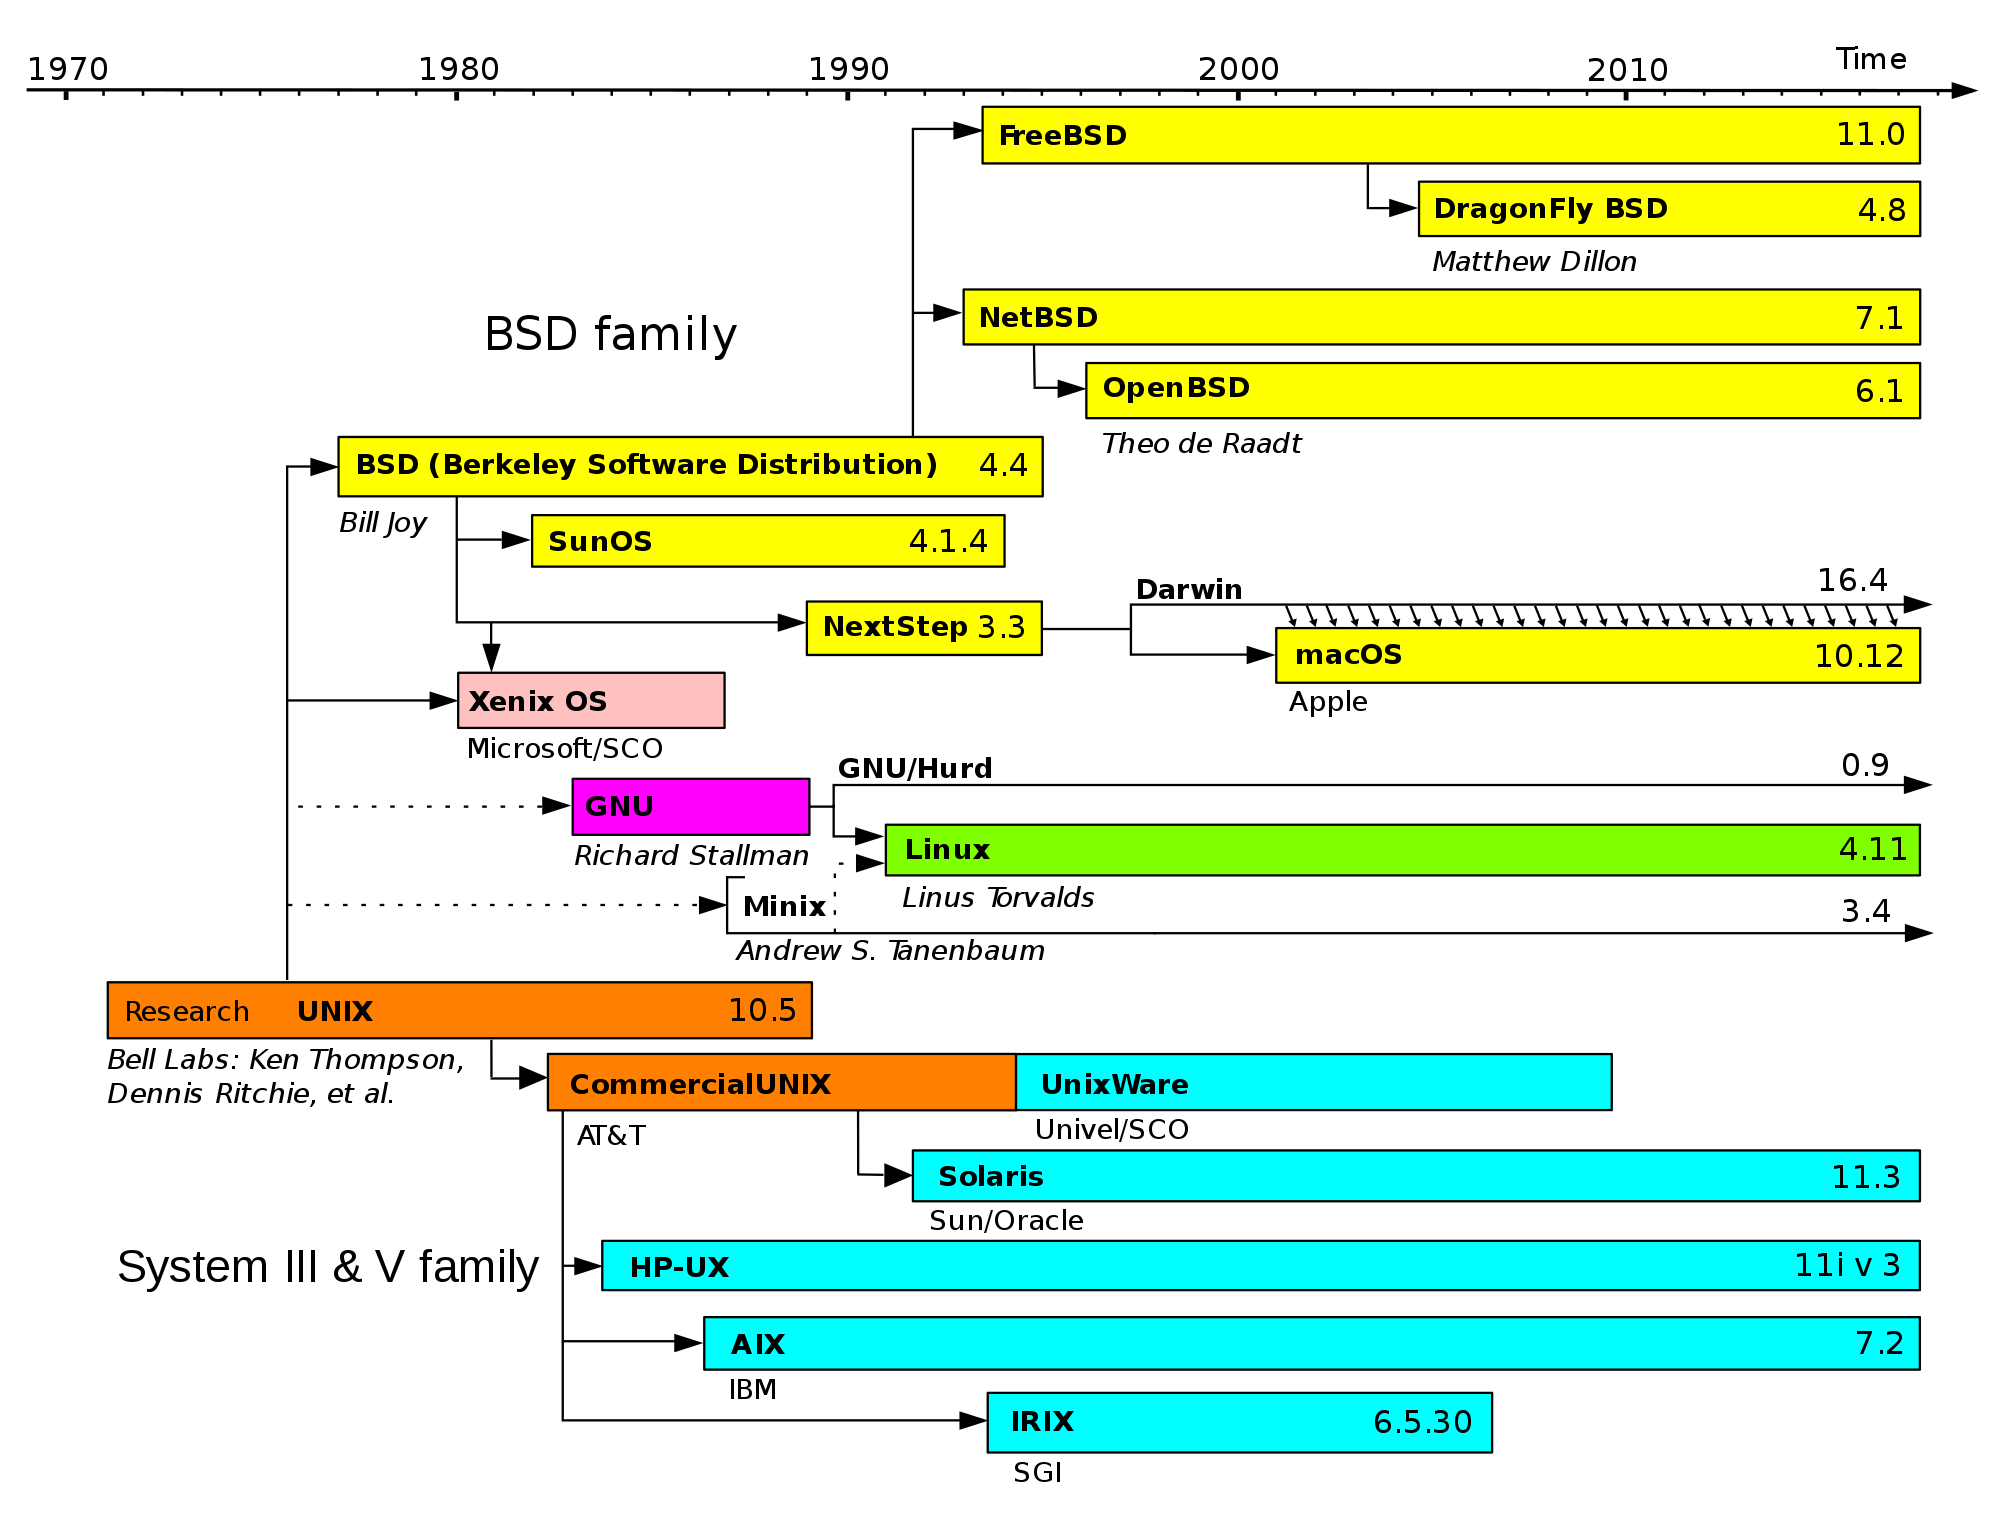
\includegraphics[width=0.6\linewidth]{unix_timeline}
  \end{center}
\end{frame}

\begin{frame}{The Unix Philosophy}
  \begin{enumerate}
    \item Write programs that do one thing and do it well.
    \item Write programs to work together.
    \item Write programs to handle text streams, because that is a universal interface.
  \end{enumerate}
\end{frame}

\section{Shell and Scripting}
\subsection{Introduction}
\begin{frame}{Introduction to Shell}
  \begin{itemize}
    \item An efficient, textual interface to your computer.
    \item Provides an interactive programming language (``scripting'').
    \item Many shells to choose from:
          \begin{itemize}
            \item Standard ones: \texttt{sh} or \texttt{bash}
            \item Shells that match languages: \texttt{csh}
            \item "Better" shells: \texttt{fish}, \texttt{zsh}, \texttt{ksh}
          \end{itemize}
    \item For this workshop, the focus is on the ubiquitous \texttt{sh} and \texttt{bash}.\footnote{Feel free to explore other shells. On macOS, many people prefer \texttt{fish} or \texttt{zsh}}
  \end{itemize}
\end{frame}

\begin{frame}{The Shell Prompt}
  \begin{itemize}
    \item What greets you when you open a terminal.
          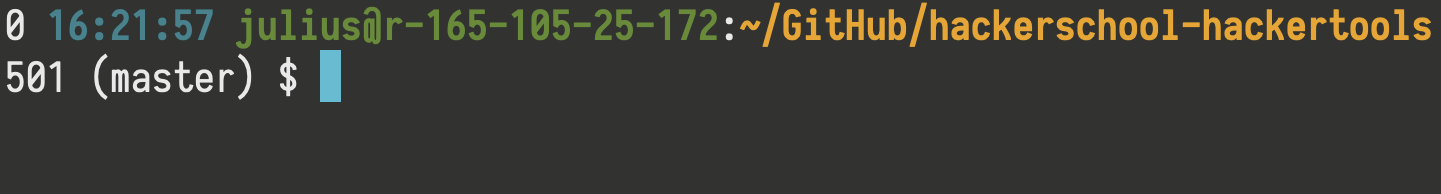
\includegraphics[width=\linewidth]{shell-prompt}
    \item Lets your run programmes and commands.
    \item Determined by the variable \mintinline{bash}{PS1}. For example, \mintinline{bash}{export PS1='> '}

  \end{itemize}
\end{frame}

\begin{frame}{Common Commands}
  \begin{itemize}
    \item \mintinline{bash}{man} to get the \textbf{man}ual pages of a command
    \item \mintinline{bash}{cd} to \textbf{c}hange \textbf{d}irectory
    \item \mintinline{bash}{ls} to \textbf{l}i\textbf{s}t files and directories
    \item \mintinline{bash}{mkdir} to \textbf{m}a\textbf{k}e \textbf{dir}ectory
    \item \mintinline{bash}{rm} to \textbf{r}e\textbf{m}ove files and directories
    \item \mintinline{bash}{cp} to \textbf{c}o\textbf{p}y file
    \item \mintinline{bash}{mv} to \textbf{m}o\textbf{v}e file
  \end{itemize}
\end{frame}

\begin{frame}{Command Editing Shortcuts}
  \texttt{bash} has shortcuts based on \texttt{emacs} keybindings:
  \begin{itemize}
    \item \keys{\ctrlwin + a}: beginning of line
    \item \keys{\ctrlwin + e}: end of line
    \item \keys{\Altwin + b}: move back one word
    \item \keys{\Altwin + f}: move forward one word
    \item \keys{\ctrlwin + k}: delete from cursor to the end of line
  \end{itemize}
  And some special ones:
  \begin{itemize}
    \item \keys{\ctrlwin + u}: delete from cursor to the start of line
    \item \keys{\ctrlwin + w}: delete from cursor to start of word
  \end{itemize}
\end{frame}

\begin{frame}{Command Control Shortcuts}
  \begin{itemize}
    \item \keys{\ctrlwin + c}: terminates the command
    \item \keys{\ctrlwin + z}: suspends the command (\mintinline{bash}{fg} to continue)
    \item \keys{\ctrlwin + l}: clears the screen
    \item \keys{\ctrlwin + s}: stops the output to the screen
    \item \keys{\ctrlwin + q}: allows output to the screen
  \end{itemize}
\end{frame}

\begin{frame}[fragile]{Script (1/2)}
  You can write programs directly at the prompt, or write into a file (writing scripts)
  \begin{minted}[linenos]{bash}
#!/bin/sh
echo something
\end{minted}
  \begin{itemize}
    \item Open an editor (for beginner, \mintinline{bash}{nano} is recommended), save the script as \texttt{example-script}
    \item On your shell, run \mintinline{bash}{chmod +x example-script}
    \item You can run your script as \mintinline{bash}{./example-script}
  \end{itemize}
\end{frame}

\begin{frame}[fragile]{Script (2/2)}
  \begin{minted}[linenos]{bash}
#!/bin/sh
echo something
\end{minted}
  Magic?
  \begin{itemize}
    \newsavebox\mybox
    \begin{lrbox}{\mybox}
      {\scriptsize\mintinline{bash}{#!/usr/bin/env python}}
    \end{lrbox}
    \item \mintinline{bash}{#!/bin/sh} is also known as the \textbf{shebang}, specifies the interpreter\footnote{You can use other interpreters too, e.g. \footnotesize\usebox{\mybox} for a python script.}
    \item \mintinline{bash}{echo} is a command that prints its arguments to the standard output.
  \end{itemize}
\end{frame}

\begin{frame}[fragile]{Flags (1/3)}
  \begin{itemize}
    \item Most command line utilities take parameters using \textbf{flags}.
    \item They come in short form (\texttt{-h}) and long form (\texttt{--help})
    \item Usually, running \mintinline{bash}{COMMAND -h} or \mintinline{bash}{man COMMAND} will give you a list of the flags the program takes.
    \item Short flags can be combined: \mintinline{bash}{rm -r -f} is equivalent to \mintinline{bash}{rm -rf} or \mintinline{bash}{rm -fr}
  \end{itemize}
\end{frame}

\begin{frame}[fragile]{Flags (2/3)}
  \begin{itemize}
    \item A double dash \texttt{--} is used in to signify the end of command options, after which only positional parameters are accepted.
          \begin{itemize}
            \item For example, to create a file called \texttt{-v}, Use \mintinline{bash}{touch -- -v} instead of \mintinline{bash}{touch -v}
            \item For example, to grep a file called \texttt{-v}, \mintinline{bash}{grep pattern -- -v} will work while \mintinline{bash}{grep pattern -v} will not.
          \end{itemize}
  \end{itemize}
\end{frame}

\begin{frame}[fragile]{Flags (3/3)}
  Some common flags are a de facto standard:
  \begin{itemize}
    \item \texttt{-a} commonly refers to all files (i.e. also including those that start with a period\footnote{In Unix, by convention files whose names begin with a period is hidden})
    \item \texttt{-f} usually refers to forcing something, e.g. \mintinline{bash}{rm -f}
    \item \texttt{-h} displays the help for most commands
    \item \texttt{-v} usually enables a verbose output
    \item \texttt{-V} usually prints the version of the command
  \end{itemize}
\end{frame}

\subsection{Shell Syntax}
\begin{frame}[fragile]{Running a command}
  \begin{minted}{bash}
echo Hello
\end{minted}
  \begin{itemize}
    \item \mintinline{bash}{COMMAND ARG1 ARG2 ARG3}
  \end{itemize}
\end{frame}

\begin{frame}[fragile]{Variables (1/3)}
  \begin{minted}{bash}
PS1='> '
echo location
name=Julius
echo $name
\end{minted}
  \begin{itemize}
    \item Used to store text
    \item \mintinline{bash}{name=value} to set variable
    \item \mintinline{bash}{$name} to access variable %$
  \end{itemize}
\end{frame}

\begin{frame}[fragile]{Variables (2/3)}
  There are also a number of special variables:
  \begin{itemize}
    \item \mintinline{bash}{$?}: get exit code of the previous command %$
    \item \mintinline{bash}{$1} to \mintinline{bash}{$9}: arguments to a script %$
    \item \mintinline{bash}{$0}: name of the script itself %$
    \item \mintinline{bash}{$#}: number of arguments %$
    \item \mintinline{bash}{$$}: process ID of current shell %$

  \end{itemize}
\end{frame}

\begin{frame}[fragile]{Variables (3/3)}
  Create a script \texttt{variable-example} containing the code below, then try running it with various arguments.
  \begin{minted}[linenos]{bash}
#!/bin/sh
echo $0
echo $1
echo $2
echo $#
\end{minted}

\end{frame}

\begin{frame}[fragile]{Loop (1/4)}
  Loop is used to run a command a bunch of times.

  For example:
  \begin{minted}{bash}
for i in $(seq 1 5); do echo hello; done
\end{minted}
\end{frame}

\begin{frame}[fragile]{Loop (2/4)}
  \begin{minted}{bash}
for i in $(seq 1 5); do echo hello; done
\end{minted}
  Let's unpack this!

  \mintinline{bash}{for x in list; do BODY; done}
  \begin{itemize}
    \item \mintinline{bash}{;} terminates a command -- equivalent to newline
    \item Split \mintinline{bash}{list}, assign each to \mintinline{bash}{x}, and run \mintinline{bash}{BODY}
    \item Split by ``whitespace'' -- we will get into it later
    \item Compared to C, no curly braces, instead \mintinline{bash}{do} and \mintinline{bash}{done}
  \end{itemize}
\end{frame}


\begin{frame}[fragile]{Loop (3/4)}
  \begin{minted}{bash}
for i in $(seq 1 5); do echo hello; done
\end{minted}
  Let's unpack this!

  \mintinline{bash}{$(seq 1 5)} %$
  \begin{itemize}
    \item Run the program \mintinline{bash}{seq} with arguments \texttt{1} and \texttt{5}
    \item Substitute the \mintinline{bash}{$(...)} block with the output of the program %$
    \item Equivalent to
          \begin{minted}{bash}
for i in 1 2 3 4 5; do echo hello; done
  \end{minted}
  \end{itemize}
\end{frame}

\begin{frame}[fragile]{Loop (4/4)}
  \begin{minted}{bash}
for i in $(seq 1 5); do echo hello; done
\end{minted}
  Let's unpack this!

  \mintinline{bash}{echo hello}
  \begin{itemize}
    \item Everything in a shell script is a command
    \item Here, it means run the \mintinline{bash}{echo} command, with argument \texttt{hello}.
    \item All commands are searched in \mintinline{bash}{$PATH} (colon-separated) %$
    \item Find out where a command is located by running \mintinline{bash}{which COMMAND}, e.g. \mintinline{bash}{which ls}
  \end{itemize}
\end{frame}

\begin{frame}[fragile]{Conditionals (1/2)}
  \begin{minted}{bash}
if test -d /bin; then echo true; else echo false; fi;
\end{minted}
  Let's unpack this!

  \mintinline{bash}{if CONDITION; then BODY; fi}
  \begin{itemize}
    \item \mintinline{bash}{CONDITION} is a command.
    \item If its exit code is \texttt{0} (success), then \mintinline{bash}{BODY} is run.
    \item Optionally, you can also hook in an \mintinline{bash}{else} or \mintinline{bash}{elif}
  \end{itemize}
\end{frame}

\begin{frame}[fragile]{Conditionals (2/2)}
  \begin{minted}{bash}
if test -d /bin; then echo true; else echo false; fi;
\end{minted}
  Let's unpack this!

  \mintinline{bash}{test -d /bin}
  \begin{itemize}
    \item \mintinline{bash}{test} is a program that provides various checks and comparison which exits with exit code \texttt{0} if the condition is true\footnote{Remember, you can check exit code using \mintinline{bash}{$?}}. %$
    \item Alternate syntax: \mintinline{bash}{[ condition ]}, e.g. \mintinline{bash}{[ -d /bin ]}
  \end{itemize}
\end{frame}

\begin{frame}[fragile]{Everything Together}
  Let's create a command like \mintinline{bash}{ls} that only prints directories:
  \begin{minted}[linenos]{bash}
#!/bin/sh
for f in $(ls)
do
  if test -d $f
  then
    echo dir $f
  fi
done
\end{minted}
\end{frame}

\begin{frame}{Bug!}
  Hold on! What if the directory is called "\texttt{My Documents}"?
  \begin{itemize}
    \item \mintinline{bash}{for f in $(ls)} expands to \\\mintinline{bash}{for f in My Documents} %$
    \item Will first perform the test on \texttt{My}, then on \texttt{Documents}
    \item Not what we wanted!
  \end{itemize}
\end{frame}

\begin{frame}{Argument Splitting}
  \begin{itemize}
    \item Bash splits arguments by whitespace (tab, newline, space)
    \item Same problem somewhere else: \mintinline{bash}{test -d $f} %$
    \item If \mintinline{bash}{$f} contains whitespace, \mintinline{bash}{test} will error! %$
    \item Need to use quote to handle spaces in arguments \mintinline{bash}{for f in "My Documents"}
    \item How do we fix our script?
    \item What do you think \mintinline{bash}{for f in "$(ls)"} does? %$
  \end{itemize}
\end{frame}

\begin{frame}[fragile]{Globbing (1/2)}
  \begin{itemize}
    \item \mintinline{bash}{bash} knows how to look for files using patterns:
          \begin{itemize}
            \item \mintinline{bash}{*}: any string of characters
            \item \mintinline{bash}{?}: any single character
            \item \mintinline{bash}{{a,b,c}}: any of these characters
          \end{itemize}
    \item Thus, \mintinline{bash}{for f in *} means all files in this directory
    \item When globbing, each matching file becomes its own argument
    \item However, still need to make sure to quote, e.g.\\ \mintinline{bash}{test -d "$f"} %$
  \end{itemize}
\end{frame}

\begin{frame}[fragile]{Globbing (2/2)}
  You can make advanced patterns
  \begin{itemize}
    \item \mintinline{bash}{for f in a*}: \pause all files starting with \texttt{a} in the current directory
    \item \mintinline{bash}{for f in foo/*.txt}: \pause all \texttt{.txt} files in \texttt{foo}
    \item \mintinline{bash}{for f in foo/*/p??.txt}: \pause all three-letter text files, starting with p, in subdirectories of \texttt{foo}
  \end{itemize}
\end{frame}

\begin{frame}{Other whitespace issues}
  \begin{itemize}
    \item \mintinline{bash}{if [ $foo = "bar" ]; then}: What's the issue? %$
          \pause
    \item What if \mintinline{bash}{$foo} is empty? arguments to \mintinline{bash}{[} are \texttt{=} and \texttt{bar} %$
    \item Possible workaround: \mintinline{bash}{[ x$foo = "xbar" ]}, but very hacky %$
          \pause
    \item Instead, use \mintinline{bash}{[[ CONDITION ]]}: \texttt{bash} built-in comparator that has special parsing
    \item Good news: it also allows \mintinline{bash}{&&} instead of \mintinline{bash}{-a}, \mintinline{bash}{||} instead of \mintinline{bash}{-o}, etc.
  \end{itemize}
\end{frame}

\begin{frame}{shellcheck}
  \begin{itemize}
    \item The mentioned problems are the most common bugs in shell scripts.
    \item A good tool to check for these kinds of possible bugs in your shell script: \url{https://www.shellcheck.net/}
  \end{itemize}
\end{frame}

\subsection{Composability}
\begin{frame}{Composability}
  \begin{itemize}
    \item Shell is powerful, in part because of \textbf{Composability}
    \item You can chain multiple programs together, rather than one program that does everything
    \item Remember \textbf{The Unix Philosophy}:
          \begin{enumerate}
            \item Write programs that do one thing and do it well.
            \item Write programs to work together.
            \item Write programs to handle text streams, because that is a universal interface.
          \end{enumerate}
  \end{itemize}
\end{frame}

\begin{frame}[fragile]{Pipe (1/2)}
  \begin{minted}{bash}
dmesg | tail
  \end{minted}
  Let's unpack this!

  \mintinline{bash}{a | b}
  \begin{itemize}
    \item Means run both \texttt{a} and \texttt{b}, but send all the output of \texttt{a} as input to \texttt{b}, and then print the output of \texttt{b}
  \end{itemize}
\end{frame}

\begin{frame}[fragile]{Pipe (2/2)}
  You can chain this even longer!

  \mintinline{bash}{cat /var/log/sys*log | grep Mar 23 | tail}
  \begin{itemize}
    \item \mintinline{bash}{cat /var/log/sys*log} prints the system log
    \item This output is fed into \mintinline{bash}{grep Mar 23}, which looks for all entries from today.
    \item This output is then further fed into \mintinline{bash}{tail}, which prints only the last 10 lines.
  \end{itemize}
\end{frame}

\begin{frame}[fragile]{Streams}
  \begin{itemize}
    \item All programs launched have 3 streams:
          \begin{itemize}
            \item \texttt{STDIN}: the program reads input from here
            \item \texttt{STDOUT}: the program prints to here
            \item \texttt{STDERR}: a second output that the program can choose to use.
          \end{itemize}
    \item By default, \texttt{STDIN} is your keyboard, \texttt{STDOUT} and \texttt{STDERR} are both your terminal
  \end{itemize}
\end{frame}

\begin{frame}[fragile]{Stream Redirection (1/2)}
  \begin{itemize}
    \item However, this can be changed!
    \item \mintinline{bash}{a | b}: makes \texttt{STDOUT} of \texttt{a} the \texttt{STDIN} of \texttt{b}.
    \item \mintinline{bash}{a > foo}: \texttt{STDOUT} of \texttt{a} goes to the file \texttt{foo}
    \item \mintinline{bash}{a 2> foo}: \texttt{STDERR} of \texttt{a} goes to the file \texttt{foo}
    \item \mintinline{bash}{a < foo}: \texttt{STDIN} of \texttt{a} is read from the file \texttt{foo}
    \item \mintinline{bash}{a <<< some text}: \texttt{STDIN} of \texttt{a} is read from what comes after \texttt{<<<}
  \end{itemize}
\end{frame}

\begin{frame}[fragile]{Stream Redirection (2/2)}
  \textbf{So why is this useful?} \pause

  It lets you manipulate output of a program!
  \pause
  \begin{itemize}
    \item \mintinline{bash}{ls | grep foo}: all files that contain the word \texttt{foo}
    \item \mintinline{bash}{ps | grep foo}: all processes that contain the word \texttt{foo}
    \item On Linux: \mintinline{bash}{journalctl | grep -i intel | tail -n 5}: last 5 system log messages with the word \texttt{intel} (case-insensitive)
    \item Note that this forms the basis for \textbf{data-wrangling}, which will be covered later.
  \end{itemize}
\end{frame}

\begin{frame}[fragile]{Grouping Commands}
  \mintinline{bash}{(a; b) | tac}
  \begin{itemize}
    \item Run \texttt{a}, then \texttt{b}, and send all their output to \texttt{tac}\footnote{\texttt{tac} print in reverse}
    \item For example: \mintinline{bash}{(echo qwe; echo asd; echo zxc) | tac}
  \end{itemize}
\end{frame}

\begin{frame}[fragile]{Process Substitution}
  \mintinline{bash}{b <(a)}
  \begin{itemize}
    \item Run \texttt{a}, generate a temporary file name for its output stream, and pass that filename to \texttt{b}
    \item To demonstrate: \mintinline{bash}{echo <(echo a) < (echo b)}
    \item On Linux: \mintinline{bash}{diff <(journalctl -b -1 | head -n20) <(journalctl -b -2 | head -n20)}
    \item This shows the difference between the first 20 lines of the last boot log and the one before that.
  \end{itemize}
\end{frame}

\subsection{Job and Process Control}
\begin{frame}[fragile]{Job (1/2)}
  Used to run longer-term things in the background.
  \begin{itemize}
    \item Use the \mintinline{bash}{&} suffix
          \begin{itemize}
            \item It will give back your prompt immediately.
            \item For example: \mintinline{bash}{(for i in $(seq 1 100); do echo hi; sleep 1; done) &}
            \item Note that the running program still has your terminal as \texttt{STDOUT}. Instead, can redirect \texttt{STDOUT} to file.
            \item Handy especially to run 2 programs at the same time like a server and client: \mintinline{bash}{server & client}
            \item For example: \mintinline{bash}{nc -l 1234 & nc localhost 1234 <<< test}
          \end{itemize}
  \end{itemize}
\end{frame}

\begin{frame}[fragile]{Job (2/2)}
  \begin{itemize}
    \item \mintinline{bash}{jobs}: see all jobs
    \item \mintinline{bash}{fg %JOBS}: bring the job corresponding to the id to the foreground (with no argument, bring the latest job to foreground)
    \item You can also background the current program: \texttt{\^{}Z}\footnote{\keys{\ctrlwin} is usually denoted as \^{}, thus \keys{\ctrlwin + z} is denoted as \texttt{\^{}Z}}, then run \mintinline{bash}{bg}
          \begin{itemize}
            \item \texttt{\^{}Z} stops the current process and makes it a job.
            \item \mintinline{bash}{bg} runs the last job in the background.
          \end{itemize}
    \item \mintinline{bash}{$!} is the PID of the last background process.
  \end{itemize}
\end{frame}

\begin{frame}[fragile]{Process Control (1/2)}
  \begin{itemize}
    \item \mintinline{bash}{ps}: lists running processes
          \begin{itemize}
            \item \mintinline{bash}{ps -A}: lists processes from all users
            \item Check out the man page for other arguments.
          \end{itemize}
    \item \mintinline{bash}{pgrep}: find processes by searching (like \mintinline{bash}{ps -A | grep})
          \begin{itemize}
            \item \mintinline{bash}{pgrep -f}: find processes with arguments
          \end{itemize}
    \item \mintinline{bash}{kill}: send a \emph{signal} to a process by ID (\mintinline{bash}{pkill} to search and run \mintinline{bash}{kill})
          \begin{itemize}
            \item Signal tells a process to do something
            \item \texttt{SIGKILL} (\texttt{-9} or \texttt{-KILL}): tell it to exit \emph{right now} (equivalent to \texttt{\^{}\textbackslash})
            \item \texttt{SIGTERM} (\texttt{-15} or \texttt{-TERM}): tell it to exit gracefully (equivalent to \texttt{\^{}C})
          \end{itemize}
  \end{itemize}
\end{frame}

\begin{frame}[fragile]{Process Control (2/2)}
  \begin{itemize}
    \item \mintinline{bash}{kill}: send a \emph{signal} to a process by ID (\mintinline{bash}{pkill} to search and run \mintinline{bash}{kill})
          \begin{itemize}
            \item Signal tells a process to do something
            \item Most common\footnote{Prefer \texttt{SIGTERM} over \texttt{SIGKILL}: \url{https://turnoff.us/geek/dont-sigkill/}}:
                  \begin{itemize}
                    \item \texttt{SIGKILL} (\texttt{-9} or \texttt{-KILL}): tell it to exit \emph{right now} (equivalent to \texttt{\^{}\textbackslash})
                    \item \texttt{SIGTERM} (\texttt{-15} or \texttt{-TERM}): tell it to exit gracefully (equivalent to \texttt{\^{}C})
                  \end{itemize}
          \end{itemize}
  \end{itemize}
\end{frame}

\begin{frame}{More Resources}
  \begin{itemize}
    \item If you are completely new to the shell, you might want to read a comprehensive guide, such as BashGuide\footnote{\url{http://mywiki.wooledge.org/BashGuide}}.
    \item For a more in-depth introduction, The Linux Command Line\footnote{\url{http://linuxcommand.org/tlcl.php}} is a good resource.
  \end{itemize}
\end{frame}

\subsection{Exercises}
\begin{frame}{xargs}
  \begin{itemize}
    \item Sometimes piping doesn't quite work because the command being piped into does not expect the newline separated format.
    \item For example, \texttt{file} command tells you properties of the file.
    \item Try running \mintinline{bash}{ls | file} and \mintinline{bash}{ls | xargs file}
    \item What is \mintinline{bash}{xargs} doing?
  \end{itemize}
\end{frame}

\begin{frame}{Other Exercises}
  \begin{itemize}
    \item Try running \mintinline{bash}{touch {a,b}{a,b}}, then \mintinline{bash}{ls}. What appeared?
    \item Sometimes you want to keep \texttt{STDIN} and still output to a file. Try running \mintinline{bash}{echo HELLO | tee hello.txt}
    \item Run \mintinline{bash}{echo HELLO > hello.txt}, then \mintinline{bash}{echo WORLD >> hello.txt}. What are the contents of \texttt{hello.txt}? How is \mintinline{bash}{>} different from \mintinline{bash}{>>}?
  \end{itemize}
\end{frame}

\section{Data Wrangling}
\subsection{Introduction}
\begin{frame}{What is Data Wrangling?}
  \begin{itemize}
    \item Have you ever had a bunch of text and wanted to do something with it?
    \item Great! That's \textbf{Data Wrangling}
    \item Adapting data from one format to another, until you end up with exactly what you wanted.
  \end{itemize}
\end{frame}

\begin{frame}[fragile]{Basic Data Wrangling (1/2)}
  Linux:
  \begin{minted}{bash}
journalctl | grep -i intel
  \end{minted}
  \begin{itemize}
    \item This is an example of basic data wrangling: finding all system log entries that mentions Intel
    \item Most of data wrangling is just about knowing what tools you have, and how to combine them.
    \item Remember \textbf{The Unix Philosophy}!
  \end{itemize}
\end{frame}

\begin{frame}{Basic Data Wrangling (2/2)}
  \begin{itemize}
    \item Let's start from the beginning:
          \begin{enumerate}
            \item We need a data source
            \item Something to do with it.
          \end{enumerate}
    \item A good use case is for logs, because you often want to investigate them, but reading the whole thing is not feasible.
  \end{itemize}
\end{frame}

\begin{frame}[fragile]{Data Wrangling Example (1/)}
  Let's try to figure out who is trying to log into my server.
  \begin{itemize}
    \item First, I try to look into my server's log: \\\mintinline{bash}{cat log}
    \item That's far too much stuffs!
    \item Let's limit it to \texttt{ssh} stuffs: \\\mintinline{bash}{cat log | grep sshd}
    \item That is still way more stuffs than what we wanted, and it's pretty hard to read.
  \end{itemize}
\end{frame}

\begin{frame}[fragile]{Data Wrangling Example (2/)}
  We can do better!
  \begin{minted}{bash}
cat log
| grep sshd
| grep "Accepted publickey for"
  \end{minted}
  There's still a lot of noise here.

  There are \emph{a lot} of ways to get rid of that, but let’s look at one of the most powerful tools in your toolkit: \texttt{sed}.
\end{frame}

\subsection{sed and Regular Expression (regex)}
\begin{frame}{sed? Isn't that the adjective to describe my life?}
  \begin{itemize}
    \item \texttt{sed} is a stream editor that builds on top of the old \texttt{ed}\footnote{If you're into lame computing jokes, here's a joke about \texttt{ed}: \url{https://www.gnu.org/fun/jokes/ed-msg.html}} editor
    \item In it, you basically give short commands for how to modify the file.
    \item If you use \texttt{vim}, you should be familiar with some of the commands (\texttt{ed} -> \texttt{vi} -> \texttt{vim})
    \item There are tonnes of commands, but the most common one is \texttt{s} for substitution.
  \end{itemize}
\end{frame}

\begin{frame}[fragile]{Back to Our Example}
  \begin{minted}{bash}
cat log
| grep sshd
| grep "Accepted publickey for"
| sed 's/.*Accepted publickey for //'
  \end{minted}
  \begin{itemize}
    \item Wow! It's a lot cleaner.
    \item What we just wrote was a simple \textbf{Regular Expression}
  \end{itemize}
\end{frame}

\begin{frame}{The s Command in sed}
  Syntax: \texttt{s/REGEX/SUBSTITUTION/}
  \begin{itemize}
    \item \texttt{REGEX} is the regular expression you want to search for.
    \item \texttt{SUBSTITUTION} is the text you want to substitute matching text with.
  \end{itemize}
\end{frame}

\begin{frame}{What is Regular Expression}
  \begin{itemize}
    \item It's a powerful construct that lets you match text against patterns.
    \item They are common and useful enough that it’s worthwhile to take some time to understand how they work.
    \item Usually (though not always) surrounded by \texttt{/}
    \item Most ASCII characters just carry their normal meaning, but some characters have special matching behaviour.
    \item Exactly which characters do what vary somewhat between different implementations of regular expressions, which is a source of great frustration.
  \end{itemize}
\end{frame}

\begin{frame}{List of Regex Special Characters}
  \begin{tabular}{|c|c|}
    \hline
    \textbf{Character} & \textbf{Meaning}                                            \\ \hline
    \texttt{.}         & Any single character except newline                         \\ \hline
    \texttt{*}         & Zero or more of the preceding match                         \\ \hline
    \texttt{?}         & One or more of the preceding match                          \\ \hline
    \texttt{[abc]}     & Any one character of \texttt{a}, \texttt{b}, and \texttt{c} \\ \hline
    \texttt{(RX1|RX2)} & Either something that matches \texttt{RX1} or \texttt{RX2}  \\ \hline
    \texttt{\^{}}      & The start of the line                                       \\ \hline
    \texttt{\$}        & The end of the line                                         \\ \hline
  \end{tabular}

  If you are unfamiliar with regex, there is a nice tutorial at \url{https://regexone.com/}
\end{frame}

\begin{frame}{Obsolete vs Modern Regex}
  \begin{itemize}
    \item Note that \texttt{sed}'s regex is somewhat weird and will require you to put a \texttt{\textbackslash} before most of these to give them special meaning.
    \item This is because by default \texttt{sed} is using the \emph{obsolete} regex format.
    \item You can avoid this problem by passing \texttt{-E} flag to \texttt{sed}, which tells it to switch to the \emph{modern} regex format.
    \item You can explore the differences by running \\\mintinline{bash}{man re_format}
  \end{itemize}
\end{frame}

\begin{frame}{Looking at our regex just now}
  \texttt{/.*Accepted publickey for /}

  \begin{itemize}
    \item It means any text that starts with any number of characters, followed by the literal string \texttt{"Accepted publickey for "}
    \item However, regexes are tricky.
    \item What if the username is also \texttt{"Accepted publickey for "}?
    \item Why? By default, \texttt{*} and \texttt{+} are ``greedy'' -- they will match as much text as they can
  \end{itemize}
\end{frame}

\begin{frame}[fragile]{Solution: Match the whole line}
  \begin{minted}{bash}
| sed -E 's/.*Accepted publickey for (.*) from ([0-9]{1,3}\.[0-9]{1,3}\.[0-9]{1,3}\.[0-9]{1,3}) port ([0-9]+) ssh2: RSA SHA256:.*//'
  \end{minted}
  Let's look at what's going on with a regex debugger\footnote{\url{https://regex101.com/r/wPc8Ii/3}}
\end{frame}

\begin{frame}{Explanation}
  \begin{itemize}
    \item The start is still as before.
    \item Then on any string of characters (username).
    \item Then on \texttt{from} followed by an IP address\footnote{This matches \texttt{999.999.999.999} which is not a valid IPv4 address. A regex that only matches valid address is left as an exercise}
    \item Then on \texttt{port} followed by a sequence of digits.
    \item Finally, we try to match on the suffix \texttt{ssh2: RSA SHA256:} followed by any string of characters.
    \item Notice that with this technique, a username of \texttt{Accepted publickey for} will not confuse us anymore. Can you see why?
  \end{itemize}
\end{frame}

\begin{frame}{Capture Groups}
  \begin{itemize}
    \item Oh no, the entire log is now empty.
    \item We want to keep the username
    \item Use \textbf{Capture Groups}!
    \item Any text matched by a regex surrounded by parentheses is stored in a numbered capture group.
    \item Capture group 0 is special. It is the whole text matched by the regex.
    \item These are available in the \texttt{SUBSTITUTION}\footnote{In some engines, even in the pattern itself!} as \texttt{\textbackslash 1}, \texttt{\textbackslash 2}, \texttt{\textbackslash 3}, etc.
  \end{itemize}
\end{frame}

\begin{frame}[fragile]{Using Capture Groups in sed}
  \begin{minted}{bash}
| sed -E 's/.*Accepted publickey for (.*) from ([0-9]{1,3}\.[0-9]{1,3}\.[0-9]{1,3}\.[0-9]{1,3}) port ([0-9]+) ssh2: RSA SHA256:.*/\1/'
  \end{minted}
  \begin{itemize}
    \item Note that in our current regex, capture group 1 is username, capture group 2 is IP address, capture group 3 is port number.
    \item You can try out using \texttt{\textbackslash 2} and \texttt{\textbackslash 3} instead of \texttt{\textbackslash 1}.
  \end{itemize}
\end{frame}

\begin{frame}{More on Regular Expressions}
  \begin{itemize}
    \item As you can probably imagine, you can come up with \emph{really} complicated regex.
    \item For example, there is an article on how you might match an email address\footnote{\url{https://www.regular-expressions.info/email.html}}. It's not easy\footnote{\url{http://emailregex.com/}}. People have even written tests\footnote{\url{https://fightingforalostcause.net/content/misc/2006/compare-email-regex.php}} and test matrices\footnote{\url{https://mathiasbynens.be/demo/url-regex}}
    \item Regular expressions are notoriously hard to get right, but they are also very handy to have in your toolbox!
  \end{itemize}
\end{frame}

\begin{frame}{More Regex Trivia}
  \begin{itemize}
    \item You can check for prime numbers using regex\footnote{\url{https://www.noulakaz.net/2007/03/18/a-regular-expression-to-check-for-prime-numbers/}}
    \item You can match \texttt{A B C} where $A + B = C$\footnote{\url{http://www.drregex.com/2018/11/how-to-match-b-c-where-abc-beast-reborn.html}}
    \item You can match nested brackets, e.g. to parse Lisp's s-expressions using Regex\footnote{\url{http://www.drregex.com/2017/11/match-nested-brackets-with-regex-new.html}}
    \item Note: these are more for curiosity purposes. There are usually better tools than regex, although for a quick and dirty script, regex is usually enough.
  \end{itemize}
\end{frame}

\begin{frame}[fragile]{Back to Data Wrangling}
  So now we have
  \begin{minted}{bash}
cat log
| grep sshd
| grep "Accepted publickey for"
| sed -E 's/.*Accepted publickey for (.*) from ([0-9]{1,3}\.[0-9]{1,3}\.[0-9]{1,3}\.[0-9]{1,3}) port ([0-9]+) ssh2: RSA SHA256:.*/\1/'
  \end{minted}
\end{frame}

\begin{frame}[fragile]{sed All the Way!}
  But we can do everything just with sed!
  \begin{minted}{bash}
cat log
| sed -E -e '/Accepted publickey for/!d' -e 's/.*Accepted publickey for (.*) from ([0-9]{1,3}\.[0-9]{1,3}\.[0-9]{1,3}\.[0-9]{1,3}) port ([0-9]+) ssh2: RSA SHA256:.*/\1/'
  \end{minted}
  \begin{itemize}
    \item \texttt{d} is to delete, \texttt{!} is to apply the function to the lines \textbf{not} selected by the pattern.
    \item Check out \mintinline{bash}{man sed}!
  \end{itemize}
\end{frame}

\subsection{More Advanced Data Wrangling}
\begin{frame}[fragile]{Let's look for common usernames}
  \begin{minted}{bash}
| sort | uniq -c
  \end{minted}
  \begin{itemize}
    \item \texttt{sort} will, well, sort its input.
    \item \texttt{uniq -c} will collapse consecutive lines that are the same into a single line, prefixed with a count of the number of occurrences.
  \end{itemize}
\end{frame}

\begin{frame}[fragile]{How about the most common logins?}
  We probably want to sort that too and only keep the most common logins
  \begin{minted}{bash}
| sort -nk1,1 | tail -n3
  \end{minted}
  \begin{itemize}
    \item \texttt{sort -n} sorts in numeric (instead of lexicographic) order, \texttt{-k1,1} means sort only by the first whitespace-separated column\footnote{In this \emph{particular} example, sorting by the whole line wouldn’t matter, but we’re here to learn!}.
    \item \textbf{Exercise}: what if we wanted the least common ones?\pause
    \item Either use \texttt{head} instead of \texttt{tail} or use \texttt{sort -r} which sorts in reverse order.
  \end{itemize}
\end{frame}

\begin{frame}[fragile]{We can do better}
  Okay, so that’s pretty cool, but we’d sort of like to only give the usernames, and maybe not one per line?
  \begin{minted}{bash}
| awk '{print $2}' | paste -sd, -
  \end{minted}
  Let's start with \texttt{paste}
  \begin{itemize}
    \item It lets you combine lines (\texttt{-s}) by a given single-character delimiter (\texttt{-d}), and ask it to to read from \texttt{STDIN} (\texttt{-})\footnote{Using GNU paste, the \texttt{-} can be omitted, but this is not POSIX compliant.}
    \item You can also emulate this using \mintinline{bash}{tr '\n' ','}, but this results in a trailing comma.
  \end{itemize}
\end{frame}

\begin{frame}{awk}
  \begin{itemize}
    \item A programming language that happens to be really good at processing text streams.
    \item There is \emph{a lot} to say about \texttt{awk} if you were to learn it properly, but as with many other things here, we’ll just go through the basics.
  \end{itemize}
\end{frame}

\begin{frame}{awk Syntax}
  \begin{itemize}
    \item Basic \texttt{awk} syntax: \texttt{pattern \{ block \}}
    \item \texttt{awk} takes in an optional pattern plus a block saying what to do if the pattern matches a given line.
    \item The default pattern (if no pattern is provided) matches all lines.
    \item Inside the block, \texttt{\$0} is set to the entire line's content, and \texttt{\$1} to \texttt{\$n} is set to the n-th field of that line, when separated by \texttt{awk} field separator\footnote{whitespace by default, can be changed with \texttt{-F}}.
  \end{itemize}
\end{frame}

\begin{frame}[fragile]{Our Use of awk}
  \begin{minted}{bash}
| awk '{print $2}'
  \end{minted}
  \begin{itemize}
    \item So in this case, we're saying that, for every line, print the contents of the second field, which happens to be the username.
  \end{itemize}
\end{frame}

\begin{frame}[fragile]{More fancy awk}
  Let’s compute the number of single-use usernames that start with \texttt{r} and end with \texttt{t}:
  \begin{minted}{bash}
| awk '$1 == 1 && $2 ~ /^r[^ ]*t$/ { print $2 }' | wc -l
  \end{minted}

  Let's unpack this!
  \begin{itemize}
    \item The pattern means the first field of the line should be equal to \texttt{1} (the count from \texttt{uniq -c}), and the second field should match the regex.
    \item The block says to print the second field (username)
    \item Finally, we count the number of lines in the output with \texttt{wc -l}.
  \end{itemize}
\end{frame}

\begin{frame}[fragile]{awk as a Programming Language}
  Remember that \texttt{awk} is a programming language, so we can actually not use \texttt{wc -l} at all:
  \begin{minted}{awk}
BEGIN { rows = 0 }
$1 == 1 && $2 ~ /^c[^ ]*e$/ { rows += $1 }
END { print rows }
  \end{minted}
  \begin{itemize}
    \item \texttt{BEGIN} is a pattern that matches the start of the input, and \texttt{END} matches the end.
    \item First we initialise the count to 0. The per-line block just adds the count from the first field. Then we print it out at the end.
  \end{itemize}
\end{frame}

\begin{frame}{Advanced awk}
  \begin{itemize}
    \item In fact, we could get rid of \texttt{grep} and \texttt{sed} entirely, because \texttt{awk} can do it all, but that is left as an exercise.
    \item A good resource to read is \url{https://backreference.org/2010/02/10/idiomatic-awk/}
  \end{itemize}
\end{frame}

\begin{frame}[fragile]{We can do Maths too!}
  \begin{minted}{bash}
| awk '{print $1}'
| paste -sd+ -
| bc
  \end{minted}
  \begin{itemize}
    \item \texttt{bc} is actually a calculator language.
    \item You can even run it straight from your shell and use it as a normal calculator.
    \item In this case, we are piping a mathematical expression to \texttt{bc}
  \end{itemize}
\end{frame}

\begin{frame}{Data Wrangling to Make Arguments (1/2)}
  \begin{itemize}
    \item Remember the \texttt{xargs} tool from the exercise just now?
    \item Since we can pipe data to it, we can use data wrangling to make arguments too.
    \item Say we want to delete all files that matches the regex \texttt{asd.a [0-9]\{2\}}
  \end{itemize}
  \mintinline{bash}{ls | grep -E 'asd.a [0-9]{2}' | xargs rm}

  What happened?
\end{frame}

\begin{frame}[fragile]{Data Wrangling to Make Arguments (2/2)}
  \begin{itemize}
    \item It's the annoying whitespace splitting again.
    \item A workaround is to use the null character (\texttt{\textbackslash 0}) as delimiter instead
  \end{itemize}
  \begin{minted}{bash}
ls
| grep -E 'asd.a [0-9]{2}'
| tr '\n' '\0'
| xargs -0 rm
  \end{minted}
\end{frame}

\subsection{Exercises}
\begin{frame}{Exercises (1/2)}
  \begin{itemize}
    \item How is \mintinline{bash}{sed s/REGEX/SUBSTITUTION/g} different from regular \texttt{sed}? What about \texttt{/textbackslash I} or \texttt{/textbackslash m}?
    \item To do in-place substitution it is quite tempting to do something like \mintinline{bash}{sed s/REGEX/SUBSTITUTION/ input.txt > input.txt}. However this is a bad idea, why? Is this particular to \texttt{sed}?
  \end{itemize}
\end{frame}

\begin{frame}{Exercises (2/2)}
  \begin{itemize}
    \item Find the number of words (in \mintinline{bash}{/usr/share/dict/words}) that contain at least three \texttt{a}s and don’t have \texttt{'s} ending.
    \item What are the three most common last two letters of those words?
    \item How many of those two-letter combinations are there?
    \item And for a challenge: which combinations do not occur?
          % cat /usr/share/dict/words | grep -v "\'s" | grep '.*a.*a.*a.*' | grep -E -o '.{2}$' | sort | uniq -c | sort -nk1,1 | tail -n3
          % cat /usr/share/dict/words | grep -v "\'s" | grep '.*a.*a.*a.*' | grep -E -o '.{2}$' | sort | uniq -c | sort -nk1,1 | wc -l
          % cat /usr/share/dict/words | grep -v "\'s" | grep '.*a.*a.*a.*' | grep -E -o '.{2}$' | sort | uniq | comm -1 -3 - <(echo {a..z}{a..z} | tr ' ' '\n') | paste -sd, -
  \end{itemize}
\end{frame}

\section{Conclusion}
\subsection{}
\begin{frame}
  \frametitle{Talk to us!}
  \begin{itemize}
    \item \textbf{Feedback form}: \url{https://tinyurl.com/hs2019-hackertools-1}
    \item \textbf{Upcoming hackerschool}:
          \begin{itemize}
            \item Hackertools Part Two
          \end{itemize}
  \end{itemize}
\end{frame}

\end{document}
